\documentclass[a4paper,12pt]{article}
\usepackage{booktabs}
\usepackage{amsmath}
\usepackage{hyperref}
\usepackage{geometry}
\usepackage{listings}
\usepackage{xcolor}
\usepackage{graphicx}

\lstset{
    language=Python,
    basicstyle=\ttfamily\small,
    keywordstyle=\color{blue},
    stringstyle=\color{red},
    commentstyle=\color{green},
    showstringspaces=false,
    numbers=left,
    numberstyle=\tiny\color{gray},
    breaklines=true,
    frame=single,
    captionpos=b
}

\geometry{margin=1in}

\title{Análisis de Datos del Cáncer de Pulmón NCCTG}
\author{}
\date{\today}

\begin{document}
	
	\maketitle
	
	\section*{Introducción}
	El cáncer de pulmón es una de las principales causas de mortalidad en todo el mundo, siendo responsable de millones de muertes cada año. En este contexto, los datos clínicos resultan fundamentales para entender los factores que afectan la supervivencia de los pacientes y, en última instancia, mejorar las estrategias de tratamiento. El conjunto de datos del cáncer de pulmón NCCTG proporciona información valiosa sobre pacientes con cáncer de pulmón avanzado recopilada por el Grupo de Tratamiento del Cáncer del Norte Central. Este conjunto de datos incluye tanto variables clínicas como datos autoinformados por los pacientes, lo que permite una visión integral de las condiciones de los mismos.
	
	El propósito de este análisis es explorar las características de este conjunto de datos, identificar patrones significativos y comprender cómo ciertas variables, como la edad, el sexo, las puntuaciones de rendimiento físico y la pérdida de peso, influyen en los tiempos de supervivencia. A través de este análisis, se espera contribuir a la identificación de posibles predictores de la supervivencia que podrían ser útiles en entornos clínicos y en investigaciones futuras.
	
	\section*{Descripción del Conjunto de Datos}
	El conjunto de datos contiene información detallada sobre 228 pacientes y se estructura en las siguientes variables clave:
	
	\begin{itemize}
		\item \textbf{inst}: Código de la institución donde se atendió al paciente. Esta variable permite identificar la procedencia de los datos.
		\item \textbf{time}: Tiempo de supervivencia del paciente en días desde el inicio del estudio hasta el momento del fallecimiento o censura.
		\item \textbf{status}: Estado de censura al final del estudio. Se codifica como 1 para censurado (es decir, el paciente estaba vivo al final del seguimiento) y 2 para fallecido.
		\item \textbf{age}: Edad del paciente en años al inicio del estudio. Esta variable es crucial para evaluar la influencia de la edad en la supervivencia.
		\item \textbf{sex}: Sexo del paciente, codificado como 1 para masculino y 2 para femenino.
		\item \textbf{ph.ecog}: Puntuación de rendimiento según el Índice de Rendimiento ECOG (Eastern Cooperative Oncology Group):
		\begin{itemize}
			\item 0: Asintomático.
			\item 1: Sintomático pero completamente ambulatorio.
			\item 2: En cama menos del 50\% del día.
			\item 3: En cama más del 50\% del día pero no postrado.
			\item 4: Postrado en cama.
		\end{itemize}
		\item \textbf{ph.karno}: Puntuación de rendimiento de Karnofsky asignada por el médico, que varía de 0 (muy mal estado) a 100 (excelente estado físico).
		\item \textbf{pat.karno}: Puntuación de rendimiento de Karnofsky asignada por el propio paciente, lo que permite comparar la percepción del paciente con la evaluación del médico.
		\item \textbf{meal.cal}: Cantidad de calorías consumidas durante las comidas diarias, una medida que puede reflejar el estado nutricional del paciente.
		\item \textbf{wt.loss}: Pérdida de peso en los últimos seis meses, medida en libras. Esta variable es un indicador importante del deterioro físico en pacientes con cáncer avanzado.
	\end{itemize}
	
	\section*{Contexto y Antecedentes}
	El uso de los datos clínicos para el análisis de supervivencia se ha convertido en una herramienta esencial en oncología. En particular, el conjunto de datos NCCTG fue recopilado para evaluar factores pronósticos relacionados con la supervivencia de pacientes con cáncer de pulmón avanzado. Una característica notable de este conjunto de datos es el uso de codificaciones específicas (por ejemplo, 1 y 2 para vivo y muerto, respectivamente) en lugar de las convencionales 0 y 1. Este enfoque, aunque inusual, se adoptó por motivos técnicos durante la era de las tarjetas perforadas en sistemas como el IBM 360 Fortran, donde los valores en blanco se interpretaban como ceros. Aunque estos sistemas han quedado obsoletos, las prácticas asociadas persistieron durante años.
	
	El estudio asociado con este conjunto de datos, liderado por Loprinzi et al. (1994), exploró cómo las puntuaciones de rendimiento y otras variables influían en la supervivencia. Estas puntuaciones, como las de Karnofsky y ECOG, han demostrado ser herramientas valiosas para evaluar el estado funcional de los pacientes y predecir resultados clínicos. Además, variables como la pérdida de peso y la ingesta calórica son indicadores del estado nutricional, que también juega un papel crítico en el manejo del cáncer.
	
	\section*{Objetivos del Análisis}
	Este informe tiene como objetivos:
	\begin{itemize}
		\item Resumir y describir las características principales de las variables del conjunto de datos.
		\item Identificar patrones y tendencias en los tiempos de supervivencia y los estados de censura.
		\item Evaluar la relación entre las puntuaciones de rendimiento, el estado nutricional y los resultados de supervivencia.
		\item Proporcionar una base para análisis futuros más complejos, como modelos de regresión de supervivencia.
	\end{itemize}
	
	\section*{Análisis de las variables}

	\subsection*{\underline{Inst}}

	Dado que este valor solo representa la institución donde se atendió al paciente, no se considera relevante para el análisis de supervivencia y, por lo tanto, no se incluirá en los análisis posteriores.

	\subsection*{\underline{Time}}

	La variable de tiempo de supervivencia es fundamental para el análisis de supervivencia y se presenta en días. \textbf{La Figura }\ref{fig:time_distribution} muestra un histograma de los tiempos de supervivencia, que revela una distribución asimétrica con una cola larga hacia la derecha. La mayoría de los pacientes sobrevivieron menos de 500 días, con un pico alrededor de los 200 días. La censura también es evidente en los datos, ya que hay un número significativo de pacientes cuyo tiempo de supervivencia no se conoce debido a la censura.
	
	\subsubsection*{Clasificación de la variable}

	En cuanto al tipo de variable es \textbf{cuantitativa discreta} debido a que se da en el número de días que sobrevivió el paciente y de \textbf{intervalos} ya que el 0 tiene un significado.


\subsubsection*{Medidas de tendencia central}

A continuación se presentan las medidas de tendencia central para la variable de tiempo de supervivencia:

\begin{table}[h!]
    \centering
    \begin{tabular}{|c|c|}
        \hline
        \textbf{Medida} & \textbf{Valor} \\
        \hline
        Media & 305.2325 \\
        \hline
        Moda & 163 \\
        \hline
        Mediana & 255 \\
        \hline
        Q1 (25\%) & 166 \\
        \hline
        Q3 (75\%) & 396 \\
        \hline
    \end{tabular}
    \caption{Medidas de tendencia central para el tiempo de supervivencia}
    \label{tab:medidas_tendencia_central}
\end{table}

\clearpage

\subsubsection*{Medidas de variabilidad}

A continuación se presentan las medidas de variabilidad para la variable de tiempo de supervivencia:

\begin{table}[h!]
    \centering
    \begin{tabular}{|c|c|}
        \hline
        \textbf{Medida} & \textbf{Valor} \\
        \hline
        Máximo & 1022 \\
        \hline
        Mínimo & 5 \\
        \hline
        Rango & 1017 \\
        \hline
        Varianza & 44371.54 \\
        \hline
        Desviación Estándar & 210.6455 \\
        \hline
        Coeficiente de Variación & 0.6901152 \\
        \hline
    \end{tabular}
    \caption{Medidas de variabilidad para el tiempo de supervivencia}
    \label{tab:medidas_variabilidad}
\end{table}

\subsubsection*{Prueba de Distribución}

El siguienete gráfico muestra la distribución de los tiempos de supervivencia comparada con diferentes tipos de distribución.

\begin{figure}[h]
 	\centering
 	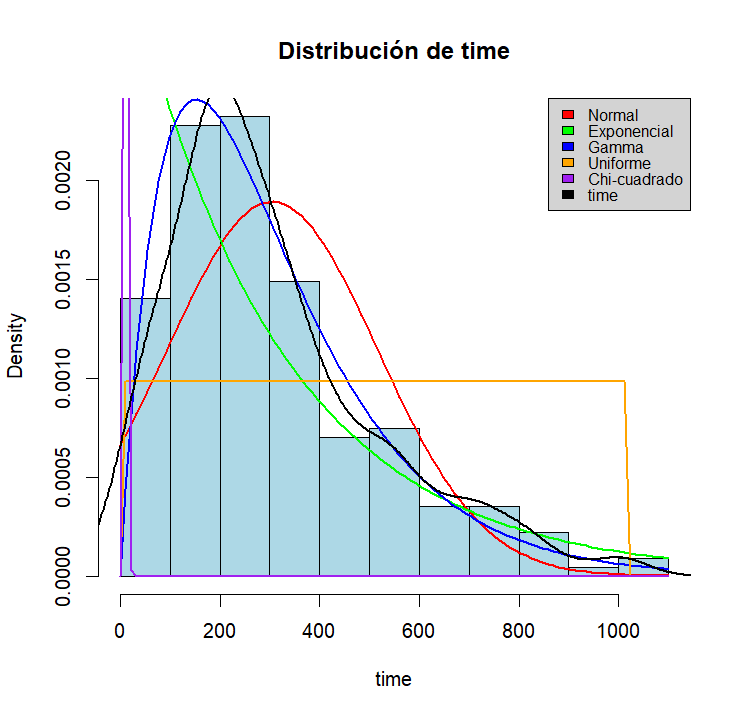
\includegraphics[width=0.7\textwidth]{distribucion_time.png}
 	\caption{Distribución de los tiempos de supervivencia}
 	\label{fig:time_distribution}
\end{figure}

Por tanto es conveniente realizar las pruebas de hipótesis para determinar si la variable sigue una distribución específica. Dicha prueba resultó en los siguientes valores:

\begin{table}[h!]
    \centering
    \begin{tabular}{|c|c|}
        \hline
        \textbf{Prueba} & \textbf{p-value} \\
        \hline
        Anderson-Darling (Normal) & 7.417945e-14 \\
        \hline
        Kolmogorov-Smirnov (Normal) & 0.001288452 \\
        \hline
        Shapiro-Wilk (Normal) & 5.114211e-10 \\
        \hline
        Kolmogorov-Smirnov (Exponencial) & 2.970448e-07 \\
        \hline
        Kolmogorov-Smirnov (Gamma) & 0.3606842 \\
        \hline
        Kolmogorov-Smirnov (Chi-cuadrado) & 3.916153e-192 \\
        \hline
    \end{tabular}
    \caption{Resultados de las pruebas de distribución para la variable \textit{time}}
    \label{tab:pruebas_distribucion}
\end{table}

Como es posible apreciar solo la prueba de Kolmogorov-Smirnov para la distribución Gamma no rechaza la hipótesis nula, por lo que se puede concluir que no es posible negar la variable \textbf{time} posee una distribución Gamma y por tanto la asumiremos en el análisis siguiente.

\subsubsection*{Intervalo de confianza para la media}

El intervalo de confianza para la media de la variable \textbf{time} es de 269.2987567105341 a 341.1661555701677 con un nivel de confianza del 99\%. Esto lo podemos saber gracias al siguiente código :

\begin{lstlisting}[language=Python, caption={Código en Python para calcular el intervalo de confianza},label={lst:intervalo_confianza_normal}]
    import pandas as pd
    import numpy as np
    from scipy.stats import norm as z
    
    # Leer el archivo CSV y seleccionar la columna 'time'
    muestra = pd.read_csv('lung_dataset.csv')['time'].dropna().values
    
    
    media_muestral = np.mean(muestra)
    desviacion_muestral = np.std(muestra, ddof=1)
    n = len(muestra)
    
    # Nivel de confianza y grados de libertad
    nivel_significancia = 0.01
    confianza = 1 - nivel_significancia
    

    z_critico = z.ppf(1 - nivel_significancia / 2)
    
    
    margen_error = z_critico * (desviacion_muestral / np.sqrt(n))
    limite_inferior = media_muestral - margen_error
    limite_superior = media_muestral + margen_error
    
    print(media_muestral, desviacion_muestral, (limite_inferior, limite_superior))
    \end{lstlisting}


    \subsubsection*{Hipótesis atractiva (luego creas una)}

    Se plantea que el tiempo de supervivencia de los pacientes con cáncer es de un promedio de 250 días. Probemos la veracidad de esta proposición mediante el siguiente código:

    \begin{lstlisting}[language=Python, caption={Código en Python para calcular el estadígrafo de la prueba de hipotesis},label={3st:prueba_hipotesis_time}]
        
    import math
    import pandas as pd
    from scipy.stats import t as t_dist

    muestra = pd.read_csv('lung_dataset.csv')['time'].dropna().values


    # H0: La media de la edad es <= 250
    # H1: La media de la edad es > 250
    mu_0 = 250  
    alpha = 0.01  # Nivel de significancia


    n = len(muestra)                     
    sample_mean = sum(muestra) / n       # Media muestral
    sample_std = math.sqrt(sum((x - sample_mean) ** 2 for x in muestra) / (n - 1))  
    t_stat = (sample_mean - mu_0) / (sample_std / math.sqrt(n))  

    # Grados de libertad
    df = n - 1


    t_critical = t_dist.ppf(1 - alpha, df)  

    \end{lstlisting}

    Este código nos da como resultado que se rechaza la hipótesis nula, por lo que el tiempo de supervivencia promedio de los pacientes con cáncer de pulmón es mayor a 250 días.

    \subsection*{\underline{Status}}

    La variable de estado de censura, codificada como 1 para censurado y 2 para fallecido, es crucial para el análisis de supervivencia. \textbf{La Figura }\ref{fig:status_distribution} muestra la distribución de los estados de censura en el conjunto de datos. La mayoría de los pacientes están censurados, lo que refleja la naturaleza de los estudios de supervivencia donde no todos los pacientes experimentan el evento de interés (es decir, la muerte) durante el período de seguimiento. 
    
    \subsubsection*{Clasificación de la variable}

    En cuanto al tipo de variable es \textbf{cualitativa nominal} debido a que se da en dos categorías y de \textbf{intervalos} ya que el 0 tiene un significado.

    \subsubsection*{Medidas de tendencia central}

A continuación se presentan las medidas de tendencia central para la variable de estado de censura:

\begin{table}[h!]
    \centering
    \begin{tabular}{|c|c|}
        \hline
        \textbf{Medida} & \textbf{Valor} \\
        \hline
        Media & 1.723684 \\
        \hline
        Moda & 2 \\
        \hline
        Mediana & 2 \\
        \hline
        Q1 (25\%) & 1 \\
        \hline
        Q3 (75\%) & 2 \\
        \hline
    \end{tabular}
    \caption{Medidas de tendencia central para la variable de estado de censura}
    \label{tab:medidas_tendencia_central_status}
\end{table}

\subsubsection*{Medidas de variabilidad}

A continuación se presentan las medidas de variabilidad para la variable de estado de censura:

\begin{table}[h!]
    \centering
    \begin{tabular}{|c|c|}
        \hline
        \textbf{Medida} & \textbf{Valor} \\
        \hline
        Máximo & 2 \\
        \hline
        Mínimo & 1 \\
        \hline
        Rango & 1 \\
        \hline
        Varianza & 0.200846 \\
        \hline
        Desviación Estándar & 0.448159 \\
        \hline
        Coeficiente de Variación & 0.260001 \\
        \hline
    \end{tabular}
    \caption{Medidas de variabilidad para la variable de estado de censura}
    \label{tab:medidas_variabilidad_status}
\end{table}

\newpage
\subsubsection*{Prueba de Distribución}

El siguiente gráfico muestra la distribución de los estados de censura en el conjunto de datos, este tipo de variable aleatoria es una Bernoulli ya que solo puede tomar dos valores, en este caso 1 y 2.

\begin{figure}[h]
    \centering
    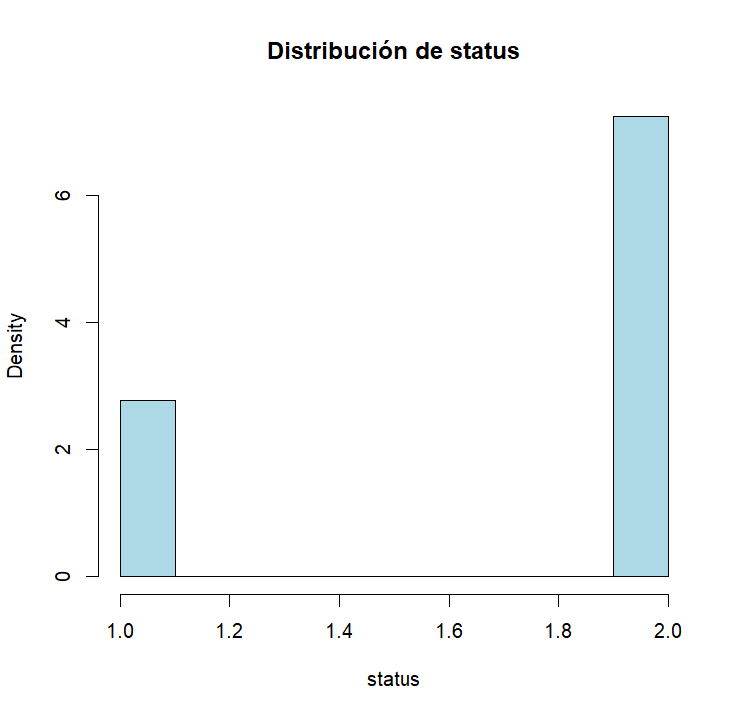
\includegraphics[width=0.7\textwidth]{distribucion_status.png}
    \caption{Distribución de los tiempos de supervivencia}
    \label{fig:status_distribution}
\end{figure}

\subsubsection*{Intervalo de confianza para la proporción}

El intervalo de confianza para la proporción de la variable \textbf{status} es de 0.6474013349555908 a 0.7999670860970408 con un nivel de confianza del 99\%. Esto lo podemos saber gracias al siguiente código:

\begin{lstlisting}[language=Python, caption={Código en Python para calcular el intervalo de confianza},label={2st:intervalo_confianza_normal}]
    import pandas as pd
    import numpy as np
    from scipy.stats import norm as z
    
    # Leer el archivo CSV y seleccionar la columna 'status'
    muestra = pd.read_csv('lung_dataset.csv')['status'].dropna().values
    
    n = len(muestra)
    proporcion_fallecidos = np.sum(muestra == 2) / n
    
    # Nivel de confianza
    nivel_significancia = 0.01
    confianza = 1 - nivel_significancia
    
    z_critico = z.ppf(1 - nivel_significancia / 2)

    margen_error = z_critico * np.sqrt(proporcion_fallecidos * (1 - proporcion_fallecidos) / n)
    
    limite_inferior = proporcion_fallecidos - margen_error
    limite_superior = proporcion_fallecidos + margen_error

    print(f"Intervalo de confianza al {confianza*100}%: ({limite_inferior}, {limite_superior})")

\end{lstlisting}

    \subsection*{\underline{Age}}

    La edad del paciente al inicio del estudio es una variable importante para evaluar la influencia de la edad en la supervivencia. \textbf{La Figura }\ref{fig:age_distribution} muestra un histograma de las edades de los pacientes, que revela una distribución aproximadamente simétrica con un pico alrededor de los 65 años.
	
    \subsubsection*{Clasificación de la variable}

    En cuanto al tipo de variable es \textbf{cuantitativa discreta} debido a que se da en el número de años que tiene el paciente y de \textbf{intervalos} ya que el 0 tiene un significado.    

    \subsubsection*{Medidas de tendencia central}

    A continuación se presentan las medidas de tendencia central para la variable de edad:
    
    \begin{table}[h!]
        \centering
        \begin{tabular}{|c|c|}
            \hline
            \textbf{Medida} & \textbf{Valor} \\
            \hline
            Media & 62.44737 \\
            \hline
            Moda & 60 \\
            \hline
            Mediana & 63 \\
            \hline
            Q1 (25\%) & 56 \\
            \hline
            Q3 (75\%) & 69 \\
            \hline
        \end{tabular}
        \caption{Medidas de tendencia central para la variable de edad}
        \label{tab:medidas_tendencia_central_edad}
    \end{table}
    
    \newpage
    \subsubsection*{Medidas de variabilidad}
    
    A continuación se presentan las medidas de variabilidad para la variable de edad:
    
    \begin{table}[h!]
        \centering
        \begin{tabular}{|c|c|}
            \hline
            \textbf{Medida} & \textbf{Valor} \\
            \hline
            Máximo & 82 \\
            \hline
            Mínimo & 39 \\
            \hline
            Rango & 43 \\
            \hline
            Varianza & 82.3276142 \\
            \hline
            Desviación Estándar & 9.0734566 \\
            \hline
            Coeficiente de Variación & 0.1452977 \\
            \hline
        \end{tabular}
        \caption{Medidas de variabilidad para la variable de edad}
        \label{tab:medidas_variabilidad_edad}
    \end{table}

    \subsubsection*{Prueba de Distribución}

    El siguiente gráfico muestra la distribución de las edades de los pacientes comparada con diferentes tipos de distribución.

 \begin{figure}[h]
 	\centering
 	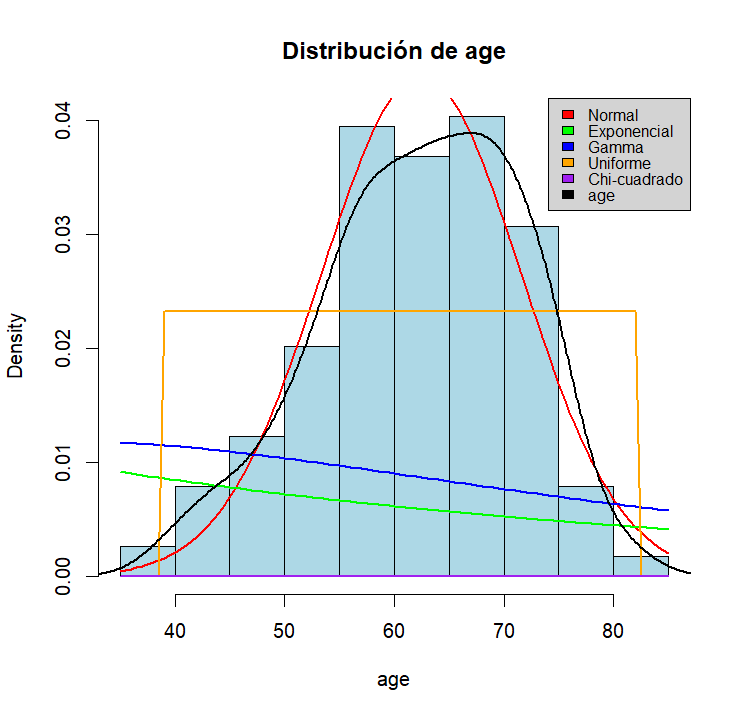
\includegraphics[width=0.7\textwidth]{distribucion_age.png}
 	\caption{Distribución de la edad de los pacientes}
 	\label{fig:age_distribution}
 \end{figure}

Por tanto es conveniente realizar las pruebas de hipótesis para determinar si la variable
sigue una distribución específica. Dicha prueba resultó en los siguientes valores:

\begin{table}[h!]
    \centering
    \begin{tabular}{|c|c|}
        \hline
        \textbf{Prueba} & \textbf{p-value} \\
        \hline
        Anderson-Darling (Normal) & 0.009280497 \\
        \hline
        Kolmogorov-Smirnov (Normal) & 0.2508968 \\
        \hline
        Shapiro-Wilk (Normal) & 0.00482907 \\
        \hline
        Kolmogorov-Smirnov (Exponencial) & 6.191832e-46 \\
        \hline
        Kolmogorov-Smirnov (Gamma) & 4.863935e-31 \\
        \hline
        Kolmogorov-Smirnov (Chi-cuadrado) & 1.831273e-198 \\
        \hline
    \end{tabular}
    \caption{Resultados de las pruebas de distribución para la variable \textit{age}}
    \label{tab:pruebas_distribucion_age}
\end{table}

    Como es posible apreciar bajo un nivel de significancia de 0.01 la prueba de Kolmogorov - Smirnov para la distribución normal no rechaza la hipótesis nula, por lo que se puede concluir que no es posible negar que la variable \textbf{age} posee una distribución normal y por tanto la  asumiremos en el análisis siguienete.
    
    \subsubsection*{Intervalo de confianza para la media}

    El intervalo de confianza para la media de la variable \textbf{age} es de 60.89954141062864 a 63.99519543147662 con un nivel de confianza del 99\%. Esto lo podemos saber gracias al siguiente código, al ser análogo al código \ref{lst:intervalo_confianza_normal} utilizado para el intervalo de confianza de la variable \textbf{time} solamente sustituiríamos:

    \begin{lstlisting}[language=Python, caption={Código en Python para calcular el intervalo de confianza}]
muestra = pd.read_csv('lung_dataset.csv')['age'].dropna().values
    
    \end{lstlisting}

    \subsubsection*{Prueba de hipótesis para la media}

    Se plantea que la edad promedio de los pacientes con cáncer es de más de 60 años. Utilizando la implementación análoga para la variable time \ref{3st:prueba_hipotesis_time}.

    \begin{lstlisting}[language=Python, caption={Código en Python para calcular el estimador de la prueba de hipotesis},label={3st:prueba_hipotesis_age}]
        

muestra = pd.read_csv('lung_dataset.csv')['age'].dropna().values

# H0: La media de la edad es <= 60
# H1: La media de la edad es > 60
mu_0 = 60  

    \end{lstlisting}

    Este código nos da como resultado que se rechaza la hipótesis nula, por lo que la edad promedio de los pacientes con cáncer de pulmón es más de 60 años. 

    \subsection*{\underline{Sex}}

    La variable de sexo del paciente, codificada como 1 para masculino y 2 para femenino, es un factor importante a considerar en el análisis de supervivencia.

    \subsubsection*{Clasificación de la variable}

    En cuanto al tipo de variable es \textbf{cualitativa nominal} debido a que se da en dos categorías y de \textbf{intervalos} ya que el 0 tiene un significado.

    \subsubsection*{Medidas de tendencia central}

A continuación se presentan las medidas de tendencia central para la variable \textit{sex}:

\begin{table}[h!]
    \centering
    \begin{tabular}{|c|c|}
        \hline
        \textbf{Medida} & \textbf{Valor} \\
        \hline
        Media & 1.394737 \\
        \hline
        Moda & 1 \\
        \hline
        Mediana & 1 \\
        \hline
        Q1 (25\%) & 1 \\
        \hline
        Q3 (75\%) & 2 \\
        \hline
    \end{tabular}
    \caption{Medidas de tendencia central para la variable \textit{sex}}
    \label{tab:medidas_tendencia_central_sex}
\end{table}

\subsubsection*{Medidas de variabilidad}

A continuación se presentan las medidas de variabilidad para la variable \textit{sex}:

\begin{table}[h!]
    \centering
    \begin{tabular}{|c|c|}
        \hline
        \textbf{Medida} & \textbf{Valor} \\
        \hline
        Máximo & 2 \\
        \hline
        Mínimo & 1 \\
        \hline
        Rango & 1 \\
        \hline
        Varianza & 0.2399722 \\
        \hline
        Desviación Estándar & 0.4898696 \\
        \hline
        Coeficiente de Variación & 0.3512272 \\
        \hline
    \end{tabular}
    \caption{Medidas de variabilidad para la variable \textit{sex}}
    \label{tab:medidas_variabilidad_sex}
\end{table}
    
 \newpage

    \subsubsection*{Prueba de Distribución}

    \textbf{La Figura }\ref{fig:sex_distribution} muestra la distribución de los pacientes por sexo. Como se puede observar, hay una proporción ligeramente mayor de pacientes masculinos en comparación con los femeninos. Esta diferencia en la distribución de sexos puede influir en los resultados de supervivencia y, por lo tanto, es crucial tenerla en cuenta en cualquier análisis posterior.

    \begin{figure}[h]
        \centering
        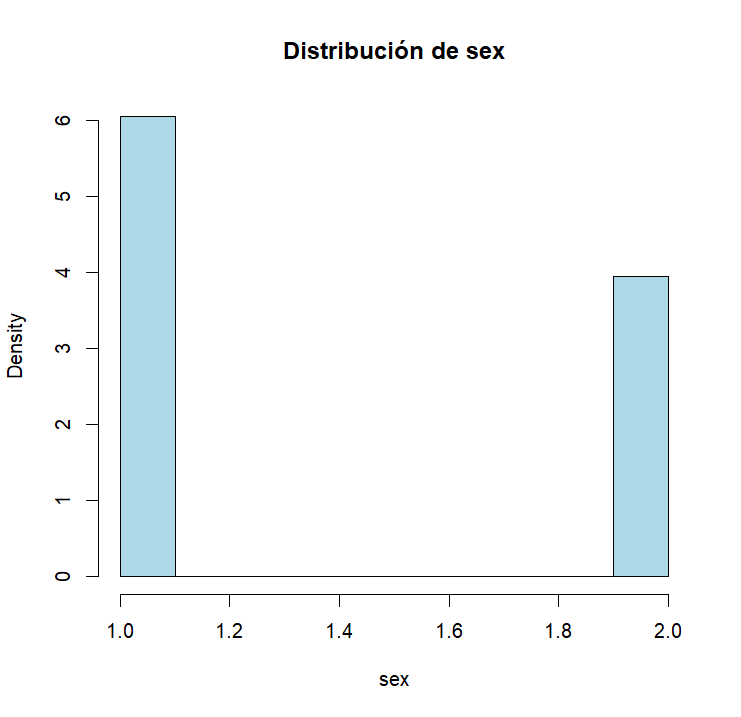
\includegraphics[width=0.7\textwidth]{distribucion_sex.png}
        \caption{Distribución del género de los pacientes}
        \label{fig:sex_distribution}
    \end{figure}

    \subsubsection*{Intervalo de confianza para la proporción}

    El intervalo de confianza para la proporción de la variable \textbf{sex} es de 0.31135420869499797 a 0.47811947551552836 con un nivel de confianza del 99\%. Esto lo podemos saber gracias al siguiente código, al ser análogo al código \ref{2st:intervalo_confianza_normal} utilizado para el intervalo de confianza de la variable \textbf{status} solamente sustituiríamos:

    \begin{lstlisting}[language=Python, caption={Código en Python para calcular el intervalo de confianza}]
        muestra = pd.read_csv('lung_dataset.csv')['sex'].dropna().values

    \end{lstlisting}

    \subsubsection*{Prueba de hipótesis para dos muestras}

    Verificación de la existencia de una diferencia significativa en la proporción de personas fallecidas (status = 2) entre los géneros (sex: 1 para hombres, 2 para mujeres). Esto permitiría explorar si el género está asociado con la probabilidad de fallecimiento en el contexto del estudio. Nos apoyaremos en el siguiente código para darle solución a la proposición.

    \begin{lstlisting}[language=Python]
        
        import math
from scipy.stats import norm
import pandas as pd

# Datos del dataset
# Status = 2 (Fallecidos)
# Sex = 1 (Hombres), 2 (Mujeres)

# Leer el archivo CSV y seleccionar las columnas necesarias
lung_data = pd.read_csv('lung_dataset.csv')[['sex', 'status']].dropna()

# Contar fallecidos y totales para hombres y mujeres
male_fallecidos = lung_data[(lung_data['sex'] == 1) & (lung_data['status'] == 2)].shape[0]
female_fallecidos = lung_data[(lung_data['sex'] == 2) & (lung_data['status'] == 2)].shape[0]
male_total = lung_data[lung_data['sex'] == 1].shape[0]
female_total = lung_data[lung_data['sex'] == 2].shape[0]

# Proporciones de fallecidos para hombres y mujeres
p_male = male_fallecidos / male_total
p_female = female_fallecidos / female_total

p_pool = (male_fallecidos + female_fallecidos) / (male_total + female_total)

z_stat = (p_male - p_female) / math.sqrt(
    p_pool * (1 - p_pool) * (1 / male_total + 1 / female_total)
)

alpha = 0.05
z_critical = norm.ppf(1 - alpha / 2)


    \end{lstlisting}

    Después de obtener los resultados del código vemos que se rechaza la hipótesis nula, por lo que hay diferencias significativas en la mortalidad entre sexos, lo cual podría tener implicaciones importantes para la investigación futura y las políticas de salud pública.

    \subsection*{\underline{Pat.karno}}

    La puntuación de rendimiento de Karnofsky asignada por el propio paciente es una medida importante del estado funcional percibido por el paciente. \textbf{La Figura }\ref{fig:pat.karno} muestra un histograma de las puntuaciones de rendimiento de Karnofsky asignadas por los pacientes, que revela una distribución asimétrica con un pico alrededor de 80-90. Las puntuaciones de rendimiento de Karnofsky asignadas por los pacientes pueden diferir de las asignadas por los médicos y pueden proporcionar información adicional sobre la percepción del paciente sobre su estado funcional.

    \subsubsection*{Clasificación de la variable}

    En cuanto al tipo de variable es \textbf{cuantitativa discreta} debido a que se da en el número de puntos asignados por el paciente de 0 a 100 y de \textbf{intervalos} ya que el 0 tiene un significado.

    \subsubsection*{Medidas de tendencia central}

    A continuación se presentan las medidas de tendencia central para la variable \textit{pat.karno}:
    
    \begin{table}[h!]
        \centering
        \begin{tabular}{|c|c|}
            \hline
            \textbf{Medida} & \textbf{Valor} \\
            \hline
            Media & 79.95556 \\
            \hline
            Moda & 90 \\
            \hline
            Mediana & 80 \\
            \hline
            Q1 (25\%) & 70 \\
            \hline
            Q3 (75\%) & 90 \\
            \hline
        \end{tabular}
        \caption{Medidas de tendencia central para la variable \textit{pat.karno}}
        \label{tab:medidas_tendencia_central_pat_karno}
    \end{table}

    \subsubsection*{Medidas de variabilidad}
    
    A continuación se presentan las medidas de variabilidad para la variable \textit{pat.karno}:
    
    \begin{table}[h!]
        \centering
        \begin{tabular}{|c|c|}
            \hline
            \textbf{Medida} & \textbf{Valor} \\
            \hline
            Máximo & 100 \\
            \hline
            Mínimo & 30 \\
            \hline
            Rango & 70 \\
            \hline
            Varianza & 213.8373016 \\
            \hline
            Desviación Estándar & 14.6231769 \\
            \hline
            Coeficiente de Variación & 0.1828913 \\
            \hline
        \end{tabular}
        \caption{Medidas de variabilidad para la variable \textit{pat.karno}}
        \label{tab:medidas_variabilidad_pat_karno}
    \end{table}

    \newpage

    \subsubsection*{Prueba de Distribución}

    El siguiente gráfico muestra la distribución de las puntuaciones de rendimiento de Karnofsky asignadas por los pacientes comparada con diferentes tipos de distribución.

    \begin{figure}[h]
        \centering
        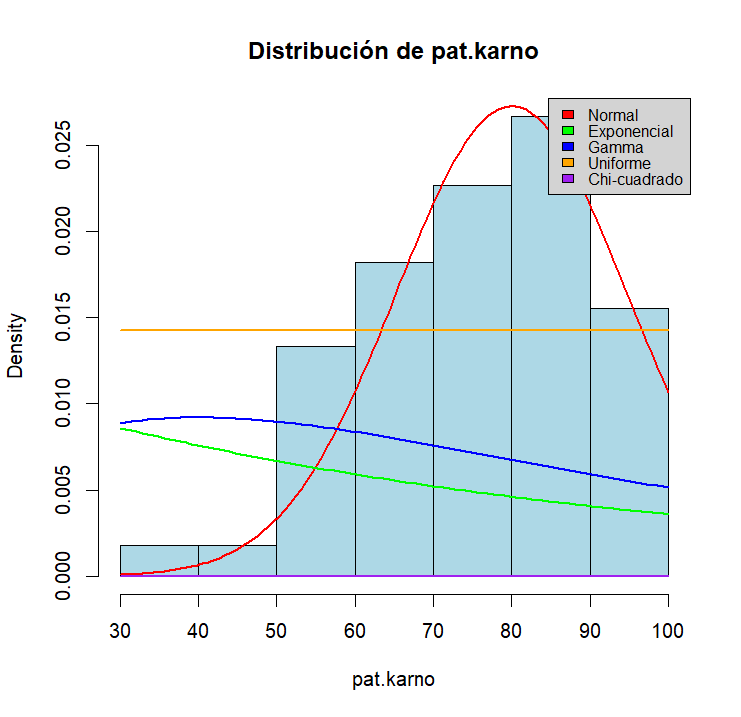
\includegraphics[width=0.7\textwidth]{distribucion_pat.karno.png}
        \caption{Distribución de las puntuaciones de rendimiento de Karnofsky asignadas por los pacientes}
        \label{fig:pat.karno}
    \end{figure}


    \subsubsection*{Intervalo de confianza para la media}

    \subsubsection*{Prueba de hipótesis para la media}

    Se plantea que la puntuación promedio asignada por los pacientes con cáncer de pulmón, en una escala de 1 a 100, en función de su bienestar corporal es de 75. Utilizando la implementación análoga para la variable time  \ref{3st:prueba_hipotesis_time}.

    \begin{lstlisting}[language=Python, caption={Código en Python para calcular el estimador de la prueba de hipotesis},label={3st:prueba_hipotesis_pat.karno}]
        
muestra = pd.read_csv('lung_dataset.csv')['pat.karno'].dropna().values

# H0: La media de la edad es <= 75
# H1: La media de la edad es > 75
mu_0 = 75  

    \end{lstlisting}

 El resultado de este código nos dice que se rechaza la hipótesis nula, por lo que la calificación que dada por cada paciente es superior a 75, lo que nos dice que en promedio los pacientes sienten mejoría ante su estado de enfermedad.
    

   

	\section*{Conclusiones}
	El conjunto de datos del cáncer de pulmón NCCTG proporciona información valiosa sobre los resultados de supervivencia en pacientes con cáncer de pulmón avanzado. Los datos destacan la importancia de las puntuaciones de rendimiento y la pérdida de peso como posibles predictores de la supervivencia. Los estudios futuros podrían utilizar este conjunto de datos para modelado pronóstico más profundo y validación de herramientas clínicas.
	
	\section*{Referencias}
	\begin{itemize}
		\item Loprinzi CL, Laurie JA, Wieand HS, Krook JE, Novotny PJ, Kugler JW, et al. "Evaluación prospectiva de variables pronósticas a partir de cuestionarios completados por los pacientes." \textit{Journal of Clinical Oncology}. 12(3):601-7, 1994.
		\item Therneau T. Documentación del paquete \textit{survival}.
	\end{itemize}
	
\end{document}
